\documentclass[10pt]{article}
\usepackage{graphicx}
\usepackage[T1]{fontenc}
\usepackage{txfonts}
\setcounter{secnumdepth}{0}
\usepackage[affil-it]{authblk}   % author affiliation
\usepackage{lineno} %line numbers
\usepackage[a4paper, total={6.5in, 8.5in}]{geometry} % set page size
\usepackage{setspace}
\usepackage{multicol}


\usepackage[authormarkup=none]{changes}
%\usepackage[final]{changes}
\definechangesauthor[name={Jess}, color=blue]{J}
\definechangesauthor[name={Iva}, color=purple]{I}
\definechangesauthor[name={Aaron}, color=green]{A}

\begin{document}

\title{Demographic Bias in Human Cell Studies }
\author{Jessica Snyder\textsuperscript{1}, Iva Bojic\textsuperscript{1,2}, Aarom Gerow\textsuperscript{3}, Carlo Ratti  \textsuperscript{1,2 } \\ \textsuperscript{1}Massachusetts Institute of Technology, SENSEable City Lab \\ \textsuperscript{2}Singapore-MIT Alliance for Research and Technology \\  \textsuperscript{3}University of Chicago, Computation Institute }

\maketitle 

\begin{multicols}{2}
Breast cancer treatments are shaped by the medical research tools used to discover the characteristics of the disease. Our question is how representative are the medical research tools, specifically human cell lines, of the breast cancer population? We find a dependence on standards, which reinforces a bias for the majority patient ethnicity. 

Female breast cancer patients became a smaller and smaller percentage of the entire female population from 1999 to 2013, figure 1A. The population-level decrease indicates environmental stressors triggering breast cancer were being reduced. One theory is the decreased prescription of a hormone-replacement therapy (HRT) shown to increase white and hispanic patient's risk of breast cancer by >20\% \cite{million2003breast}. HRT use was not found to increase black woman's risk. Since HRTs were limited in 2002, breast cancer incidence rates among white, hispanic and Native American woman have fallen, while the rate for black and Asian women increased over the same time. Grouping the breast cancer population by ethnicity exposes breast cancer as a heterogenous disease, with many sub-types, each with their own set of risk factors and pathologies. 

The prognosis for all women diagnosed with breast cancer has improved, in part due to advances in screening, detecting tumors earlier, increasing survival rates, especially for women under 50 years old \cite{etzioni2003case}. Of the deaths caused by breast cancer, black woman had the highest rate of death from 1999-2013, higher than white women, who are more likely to be diagnosed, figure 1B. Possible explanations include diagnosis at later stage and faster growing, more aggressive, tumor sub-types, both of which disproportionately affect black patients \cite{batina2013variation}. 

Characterization of each breast cancer sub-type provides the scientific basis for treatment options, as it already has for the most common forms as shown by the increasing survival rate. Our question is, which ethnicities, as a proxy for tumor sub-types, have been included in medical research, specifically breast cancer cell lines? 

A master list of cell names was previously curated to study cell line authentication and quality control, fully annotated with donor age, gender and ethnicity \cite{yu2015resource}. Analysis of the bank of human cell lines shows cell lines are used as standards, as intended. The first breast cancer cell line was donated by a 74 years old female patient in 1958, named BT-20. BT-20 remained the only breast cancer cell lines for more than a decade, until other cell lines were added from subsequent white female patients in the 1970s. The first cell line derived from a black patient's biopsy was in 1974, followed by the first Asian breast cancer cell lines 20 years later in 1994 and the first Hispanic one year later in 1995. No Native American breast cancer cell lines are currently available. To date, 134 breast cancer cell lines derived from humans are available. Of which, 68 have declared an ethnicity for the donor. Of those, the donors include a majority white, 50, 12 from black donors, 4 from Asian donors, and 2 from Asian donors.

Citations of cell lines the publications reinforce standards homogenize the research focus. 1.2 million publications cited a human cell line derived from breast cancer from 1975-2016. 85.6\% cited a cell line from a declared white donor. The next most populous cell line citation was unknown donor ethnicity, 8.8\%, then black donors, 5.0\%, an order of magnitude less publications cited cell lines from Asian donors, 0.5\%, another order of magnitude less were declared Hispanic cell lines, 0.1\%, and as there are no breast cancer cell lines donated by Native American patients, there are no citations, figure 1C.

Commercialization of scientific research in the form of a patent shows progress towards a medical treatment. Analysis of the U.S. patent database from 2001 through 2015 shows the majority cell model is from a white donor, the second most being black. No other ethnicities are cited, figure 1D. 

We calculated the fraction each ethnicity represents in the incidence and death population from published U.S. CDC statistics. As well as the fraction of publications and U.S. patents which cite each ethnicity's cell line, of those publications and patents which cite any cell line. Now we compare those fractions to calculate the bias. First, is there a bias in treatment efficacy? Yes, subtracting each ethnicity's fraction in the incidence from the death population, figure 1E, shows black patient are the only ethnicity to represent more death population than incidence, by 0.4\%. Next, is there a bias in the publication record? Yes, again, blacks represent approximately 10\% more of the death population than citations of black cell lines in publications, figure 1F. White is only ethnic group represented  more in publications than the death population, by more than 15\%.  The trend continues for patents, a bias in favor of the majority ethnicity, figure 1G. Comparison of the ethnic representation in each group in 2013 shows a more than proportional representation of the majority patient ethnicity and dependence on cell model standards, figure 1H. 

The use of cell models may hinder generalization of results. More than 50,000 woman will be diagnosed with breast cancer between 2010-2020 in the US alone, costing an estimated \$48 billion in medical treatment \cite{mariotto2011projections, weir2015past}. The National Institutes of Health (NIH) and the National Cancer Institute (NCI) invested a combined \$4.1 billion in breast cancer research from 2012 through 2014, with the goal of restoring the nation's breast cancer patient population to good health. Data-driven analyses of disease burden and treatment effectiveness have been used in the past to guide medical research funding and health policy decisions towards the most productive outcomes \cite{kim2016cancer}. 

To this end, as black patients comprise more of the death population than the incidence, CDC statistics suggests that breast cancer treatment is less effective in treating black women than women of all other races. And even though previous studies showed black breast cancer patients presented elevated risk for aggressive, intrinsic factors of breast cancer \cite{huo2009population, reding2012examination}, instead of putting more resources into research using cell lines from black donors, we have just shown totally the opposite effect -- Whites are over-represent by more than 15\%.

Today the only regulative we have is the one of the US Food and Drug Administration (FDA) who recognized genetic factors sensitize pharmaceutical efficacy and responded by implementing the Demographic Rule in 1998. The rule standardizes race and ethnicity representative during clinical trails based on the target therapeutic population as identified by the drug's sponsor. However, clinical trials are just the last step of the research process which typically progresses from cell models, to animal models, and finally human models. Should we extend this regulation also to the preclinical stage?

Recent efforts from NIH to balance sex in cell and animal studies would definitely suggest so \cite{clayton2014nih}. Namely, similar to the Demographic Rule, in 1993 Congress passed the NIH Revitalization Act to increase the representation of women and minorities in clinical trials. However, despite of multiple calls for actions, publications often continued to neglect sex-based considerations and analysis in preclinical studies.

Initiatives, such as Cancer Moon Shot's database approach, catalog tumor sub-types from the patient populations, decreasing dependence on standards, highlighting the patients without effective treatment options \cite{lowy2016cancer}. We hope such collaborative approaches can populate the human cell line bank and medical research community to discover the multitude of pathologies involved in breast cancer, alleviating the community's dependence on standards as we realize the potential of personalized medicine.  
 
\end{multicols}

\begin{figure}[h!]
\centering
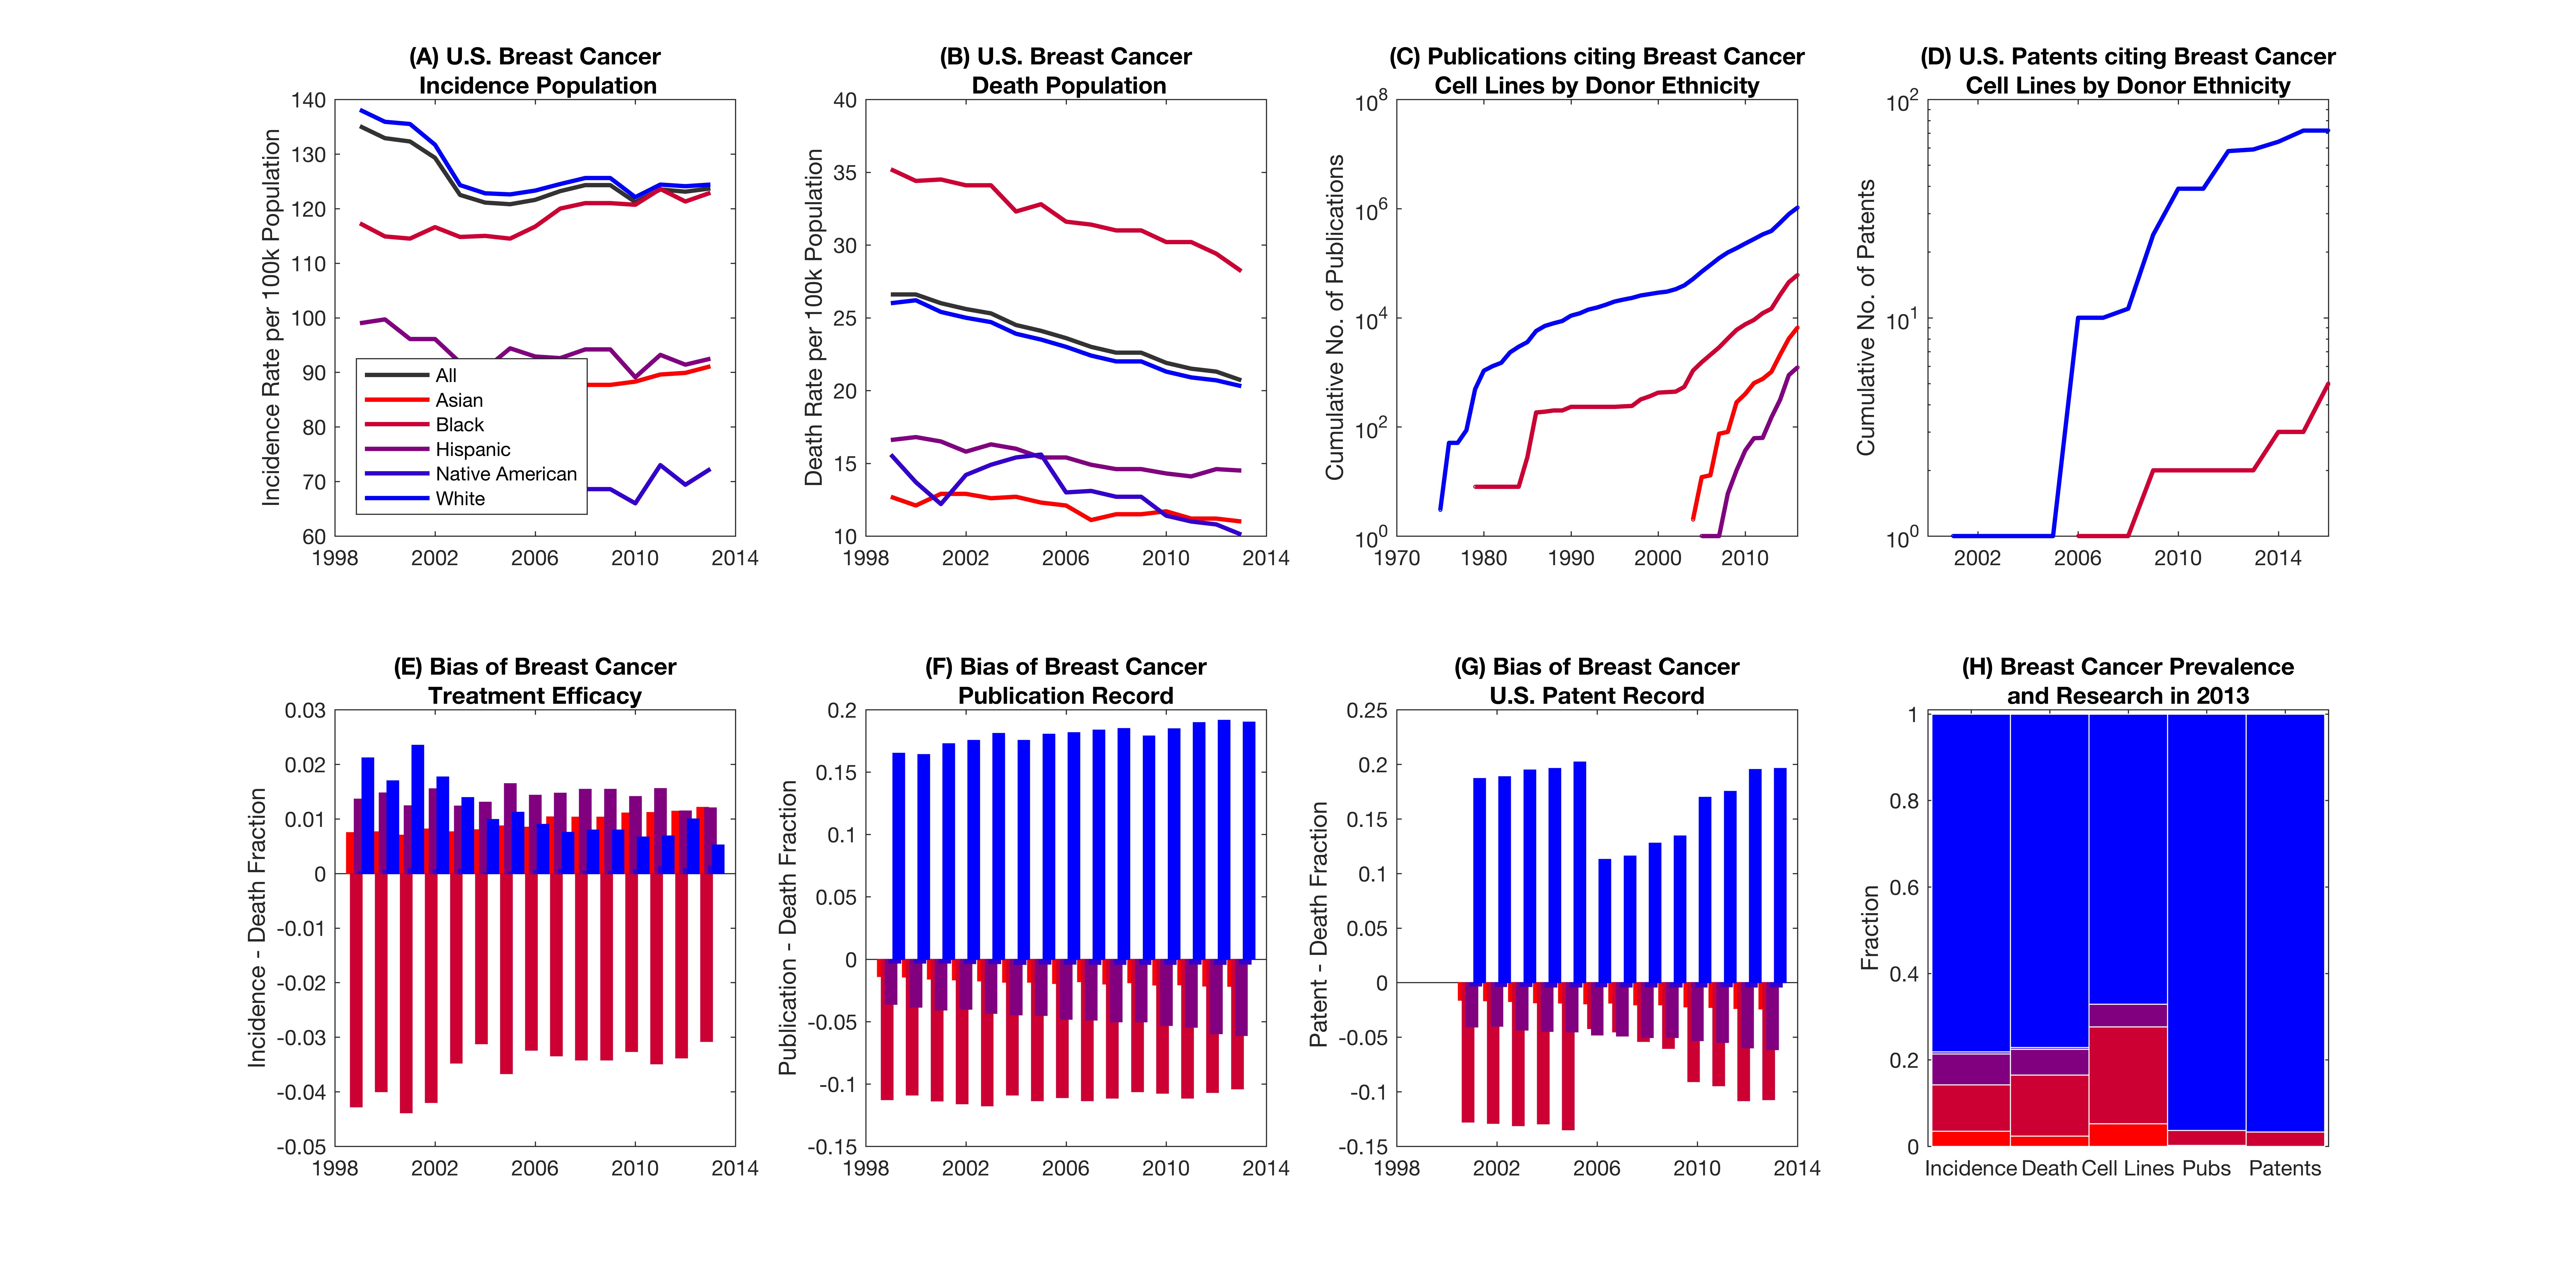
\includegraphics[width=1\columnwidth, trim = {30cm 10cm 30cm 5cm}, clip]{Figures/BreastComposite.jpg}
\caption{\label{PS2} Breast cancer prevalence and research.}
\end{figure}
 
\bibliographystyle{unsrt}
\bibliography{refs}

\section{Appendix}
The same analysis was conducted from prostate and lung cancer. 

\begin{figure}[h!]
\centering
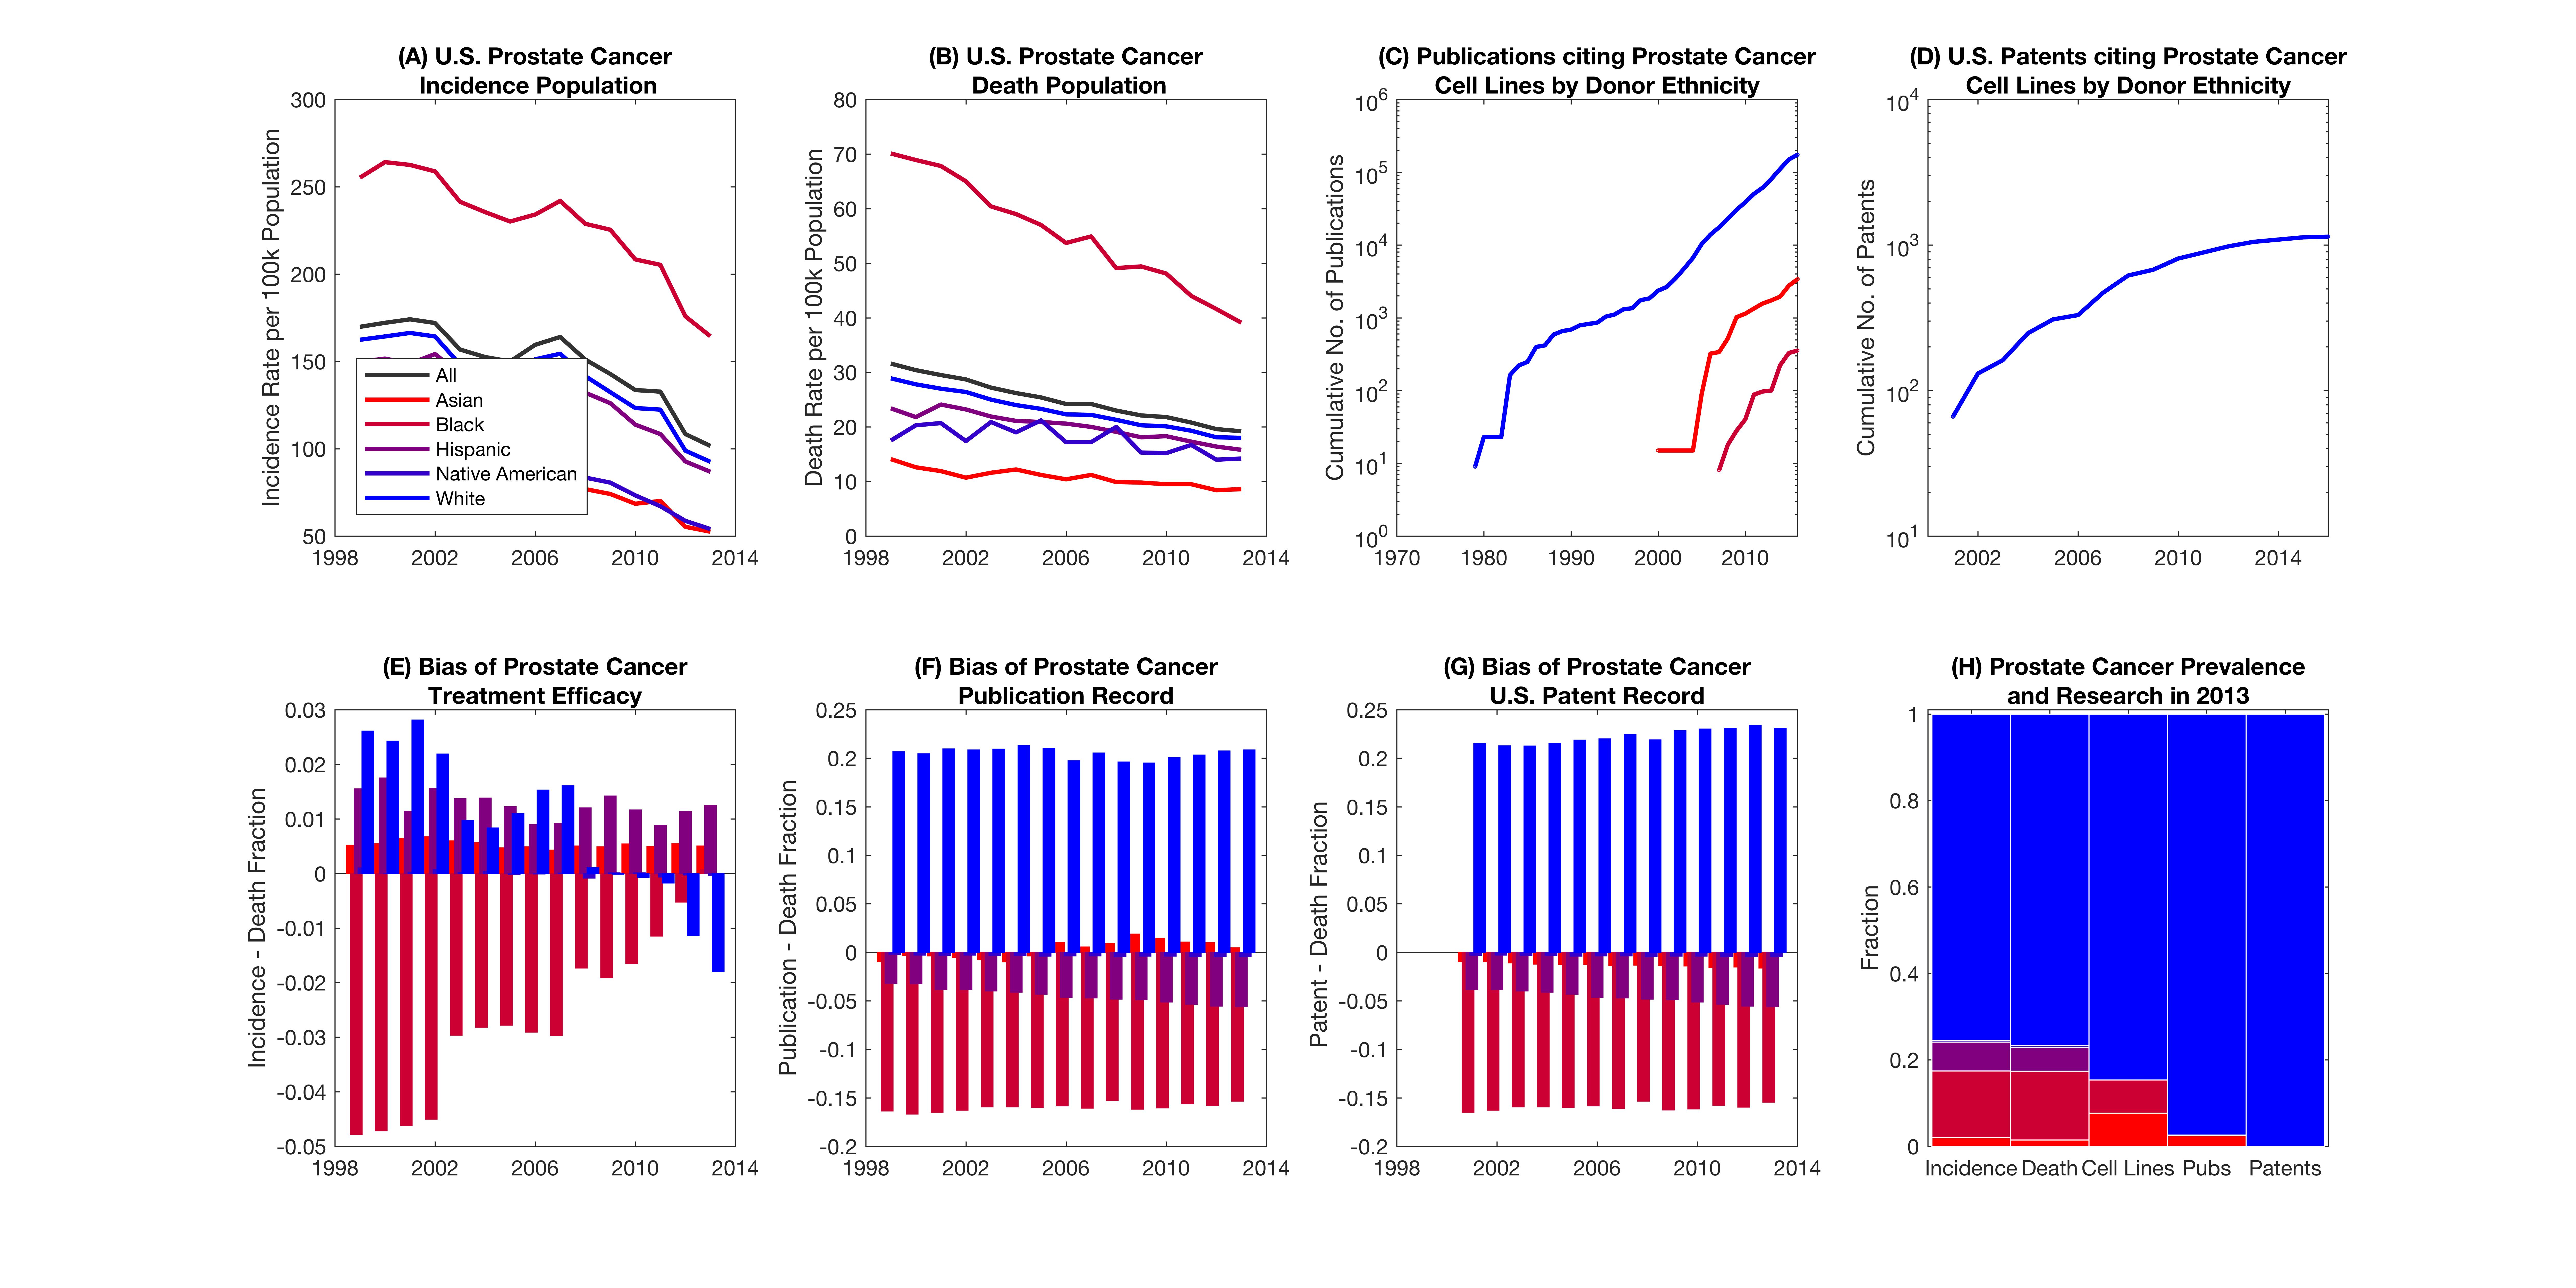
\includegraphics[width=1\columnwidth, trim = {30cm 10cm 30cm 5cm}, clip]{Figures/ProstateComposite.jpg}
\caption{\label{PS2} Prostate cancer}
\end{figure}

\begin{figure}[h!]
\centering
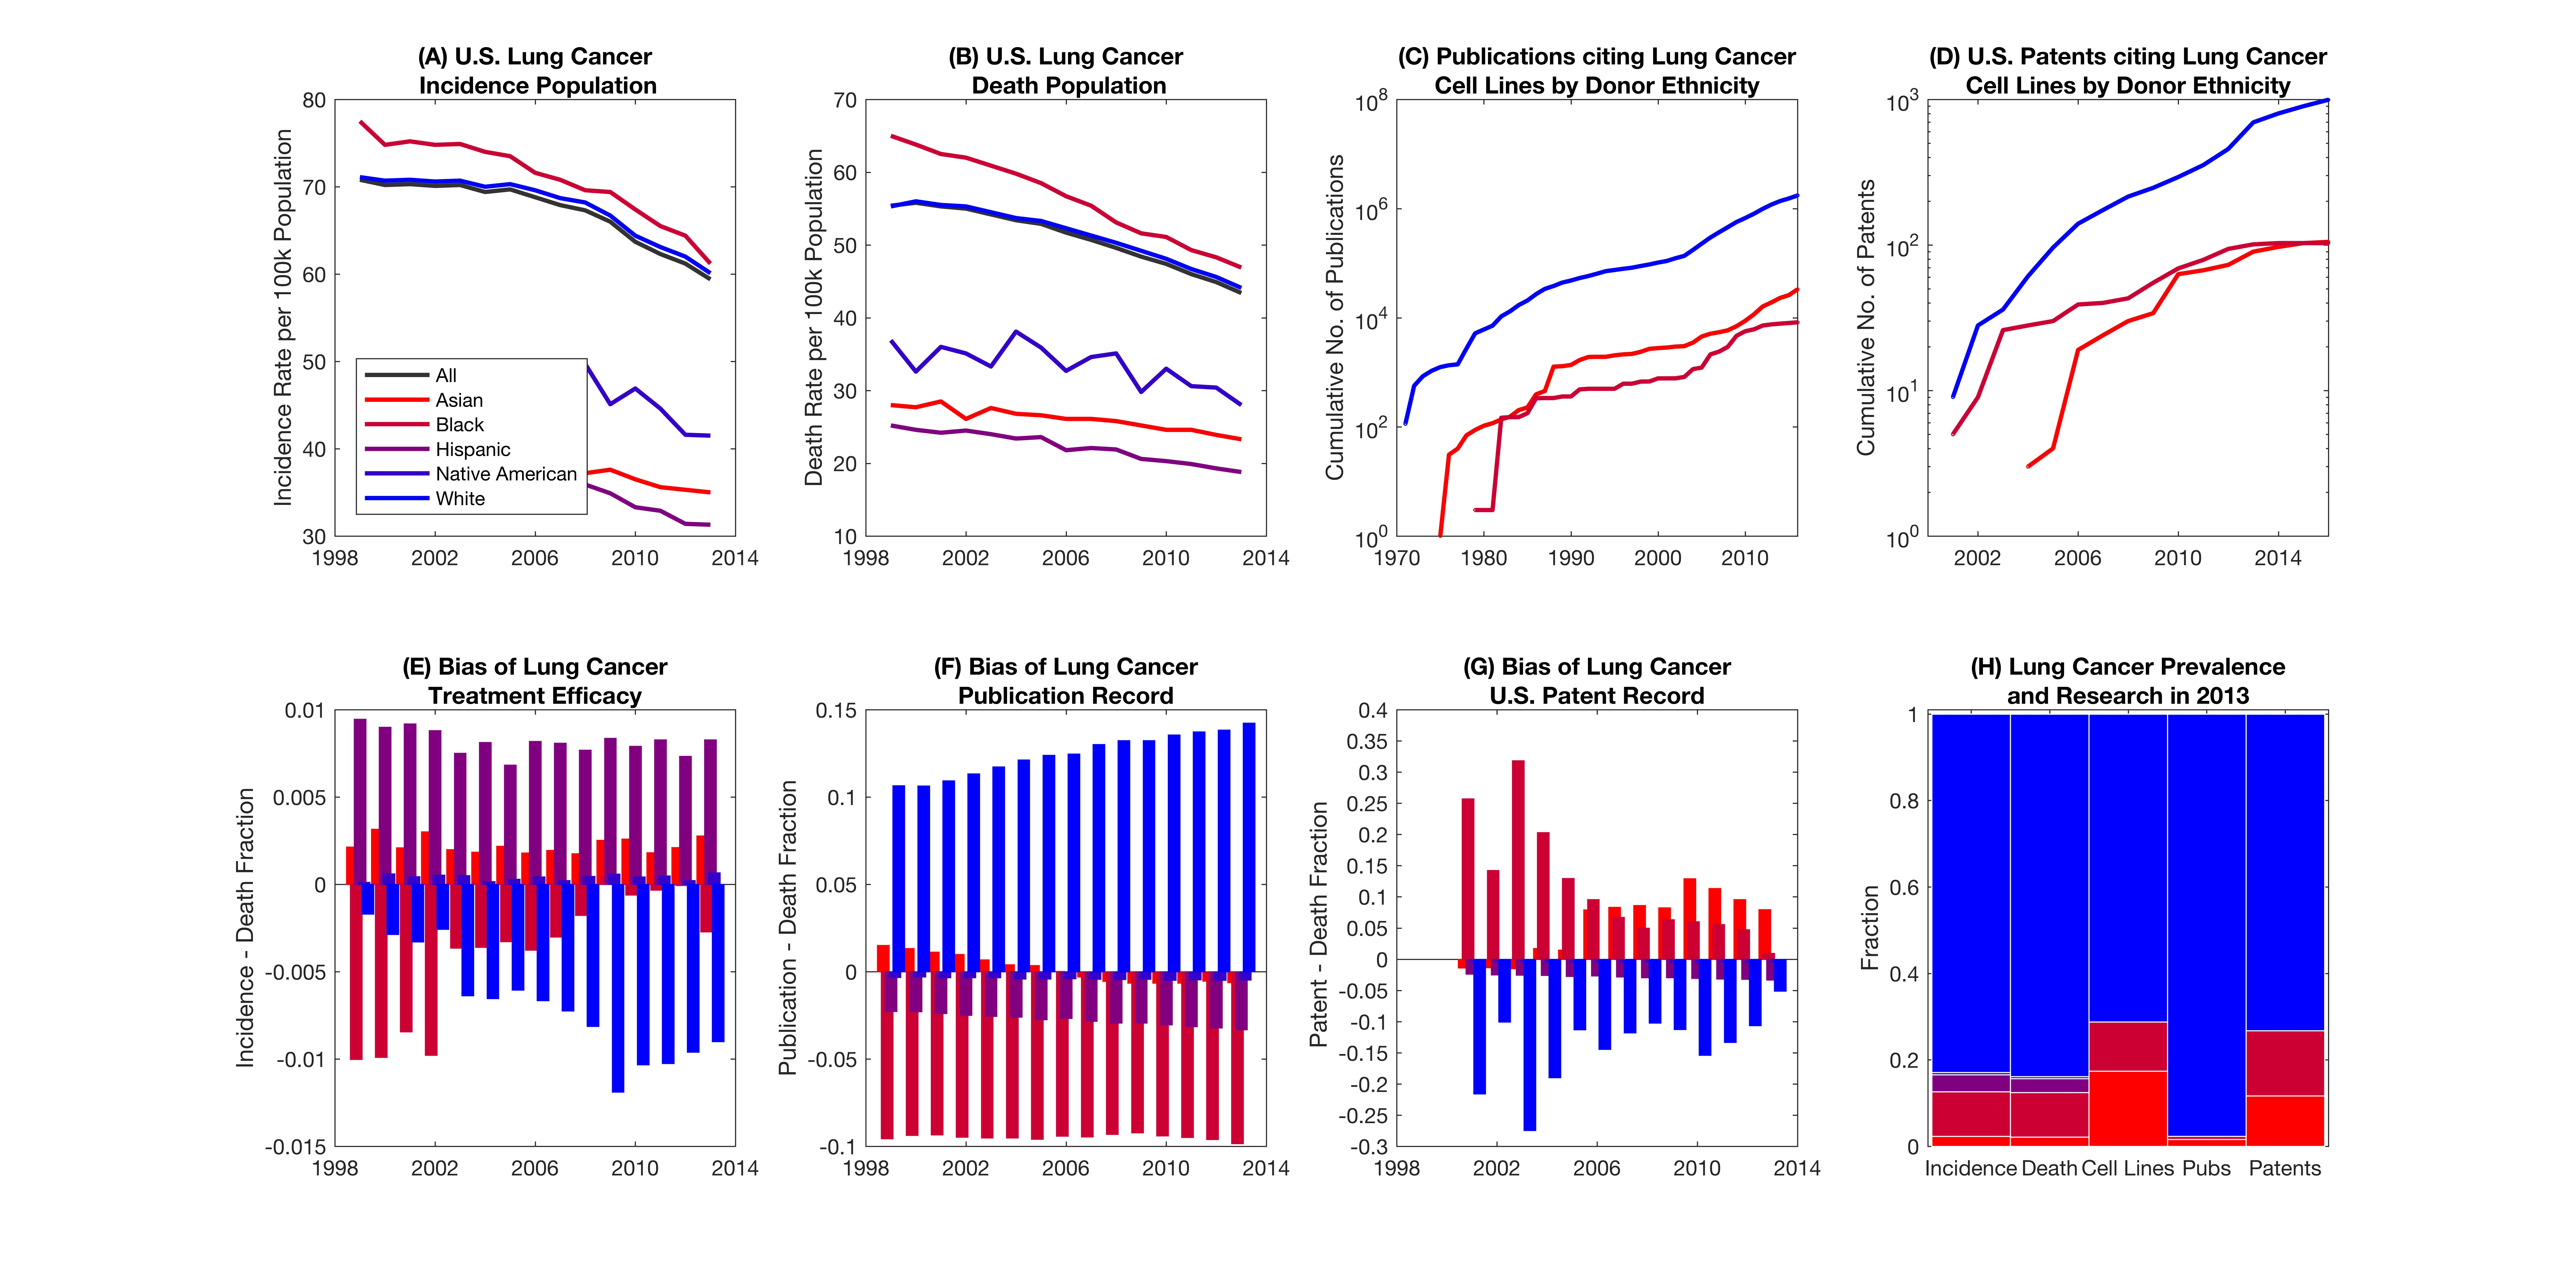
\includegraphics[width=1\columnwidth, trim = {30cm 10cm 30cm 5cm}, clip]{Figures/LungComposite.jpg}
\caption{\label{PS2}  Lung cancer.}
\end{figure}

\end{document}
